% Figure definitions live here to keep the explanatory text uncluttered.
\newcommand{\RealizationFigure}{%
\begin{figure}[htbp]\centering
\begin{tikzpicture}[x=.87cm,y=.92cm]
  \foreach \k/\style in {0/solid,1/dashed,2/densely dotted}{
    \begin{scope}[yshift=-1.13*\k cm]
      \draw[-{Latex[length=2mm]},gray!70] (0,0)--(12.4,0) node[right,font=\scriptsize] {$t$};
      \draw[black,\style,line width=1pt,samples=220,domain=0:12,smooth]
        plot (\x,{.23*sin((85+19*\k)*\x)+.13*cos((169-12*\k)*\x)+.06*sin((390+20*\k)*\x)});
      \node[left,font=\small] at (0,0) {$s_{\the\numexpr\k+1\relax}$};
    \end{scope}}
  \draw[black,densely dashed] (7.5,.55)--(7.5,-2.9);
  \node[above,font=\small] at (7.5,.55) {$t_0$};
\end{tikzpicture}
\caption{Each trace fixes an experimental outcome $s_i$ and varies time. The vertical dashed line fixes time $t_0$ and compares outcomes.}
\label{fig:realizations}\end{figure}}

\newcommand{\MarginalFigure}{%
\begin{figure}[htbp]\centering
\begin{tikzpicture}[x=.8cm,y=.84cm]
  \foreach \y/\label in {3/Persistent,1.5/Independent,0/Alternating}{
    \draw[-{Latex[length=2mm]},black!60] (.7,\y)--(10.7,\y) node[right,font=\footnotesize] {$n$};
    \node[left,font=\small] at (.5,\y) {\label};
    \draw[black!20,dotted] (.9,{\y+.34})--(10.5,{\y+.34}) (.9,{\y-.34})--(10.5,{\y-.34});}
  \foreach \n in {1,...,10} {\fill[black] (\n,3.34) circle (1.6pt);}
  \foreach \n/\v in {1/1,2/-1,3/1,4/1,5/-1,6/-1,7/1,8/-1,9/1,10/1}
    {\fill[black] (\n,{1.5+.34*\v}) circle (1.6pt);}
  \foreach \n/\v in {1/1,2/-1,3/1,4/-1,5/1,6/-1,7/1,8/-1,9/1,10/-1}
    {\fill[black] (\n,{.34*\v}) circle (1.6pt);}
  \node[right,font=\scriptsize] at (10.4,3.34) {$+1$};
  \node[right,font=\scriptsize] at (10.4,2.66) {$-1$};
\end{tikzpicture}
\caption{Illustrative realizations of three processes with the same $50$--$50$ distribution at every time. Their temporal correlations and responses to averaging differ.}
\label{fig:marginals}\end{figure}}

\newcommand{\WindowOverlapFigure}{%
\begin{figure}[!ht]\centering
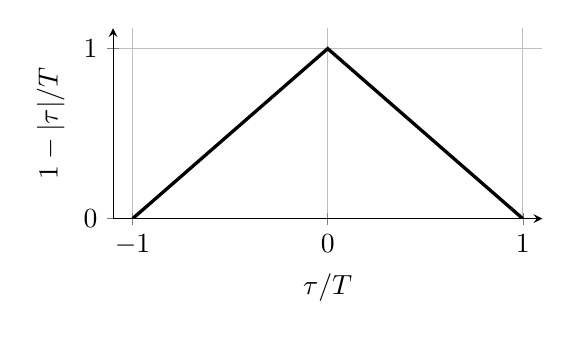
\begin{tikzpicture}
\begin{axis}[width=.58\linewidth,height=4cm,axis lines=left,
  xlabel={$\tau/T$},ylabel={$1-|\tau|/T$},
  xmin=-1.1,xmax=1.1,ymin=0,ymax=1.12,
  xtick={-1,0,1},ytick={0,1},grid=major]
  \addplot[black,very thick] coordinates {(-1,0) (0,1) (1,0)};
\end{axis}\end{tikzpicture}
\caption{The fraction of a length-$T$ observation interval shared with a copy shifted by $|\tau|$. Large lags have fewer pairs of observed samples.}
\label{fig:overlap}\end{figure}}

\newcommand{\LorentzianFigure}{%
\begin{figure}[htbp]\centering
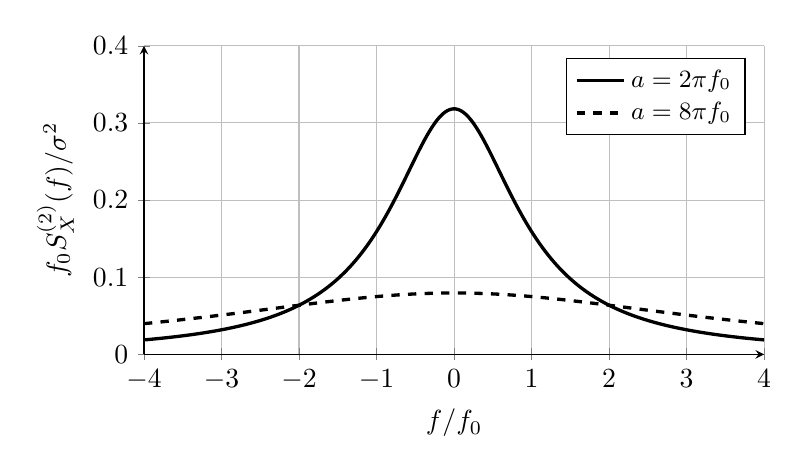
\begin{tikzpicture}
\begin{axis}[width=.78\linewidth,height=5.5cm,axis lines=left,
  xlabel={$f/f_0$},ylabel={$f_0S_X^{(2)}(f)/\sigma^2$},
  xmin=-4,xmax=4,ymin=0,ymax=.4,grid=major,
  legend style={at={(.97,.96)},anchor=north east,font=\small},samples=240]
  \addplot[black,very thick,domain=-4:4] {1/(pi*(1+x^2))};
  \addlegendentry{$a=2\pi f_0$}
  \addplot[black,very thick,dashed,domain=-4:4] {4/(pi*(16+x^2))};
  \addlegendentry{$a=8\pi f_0$}
\end{axis}
\end{tikzpicture}
\caption{Exponential correlations with the same variance $\sigma^2$, plotted using an arbitrary reference frequency $f_0>0$. Faster decorrelation ($a$ four times larger) spreads the same spectral area over a wider range of frequencies.}
\label{fig:lorentzian}\end{figure}}

\newcommand{\MatchedResistorFigure}{%
\begin{figure}[htbp]\centering
\begin{tikzpicture}[x=1cm,y=1cm,>=Latex]
  \draw (0,0)--(5.9,0);
  \draw (0,0)--(0,1.1);
  \draw (0,1.55) circle (.45);\node at (0,1.55) {$v_n$};
  \draw (0,2)--(0,2.45)--(1.82,2.45);
  \draw[decorate,decoration={zigzag,segment length=4pt,amplitude=1.7pt}]
    (1.82,2.45)--(2.38,2.45);
  \node[above] at (2.1,2.6) {$R$};
  \draw (2.38,2.45)--(5.9,2.45)--(5.9,1.55);
  \draw[decorate,decoration={zigzag,segment length=4pt,amplitude=1.7pt}]
    (5.9,1.55)--(5.9,.99);
  \draw (5.9,.99)--(5.9,0);
  \node[right] at (5.9,1.2) {$R_L=R$};
  \draw[<->,teal] (4.7,.12)--(4.7,2.32);
  \node[left,text=teal] at (4.7,1.22) {$v_L$};
\end{tikzpicture}
\caption{Matched load: half the source voltage and one quarter of its voltage-noise PSD.}
\label{fig:match}\end{figure}}

\newcommand{\NoiseBandwidthFigure}{%
\begin{figure}[htbp]\centering
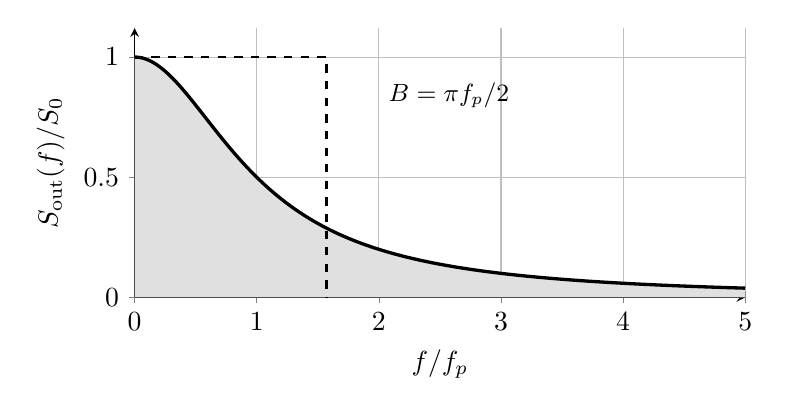
\begin{tikzpicture}
\begin{axis}[width=.77\linewidth,height=5cm,axis lines=left,
  xlabel={$f/f_p$},ylabel={$S_{\mathrm{out}}(f)/S_0$},
  xmin=0,xmax=5,ymin=0,ymax=1.12,grid=major,samples=220]
  \addplot[draw=none,fill=black!12,domain=0:5] {1/(1+x^2)} \closedcycle;
  \addplot[black,very thick,domain=0:5] {1/(1+x^2)};
  \addplot[black,dashed,thick] coordinates {(0,1) (1.5708,1) (1.5708,0)};
  \node[anchor=west,font=\small] at (axis cs:2.0,.84) {$B_{\enbw}=\pi f_p/2$};
\end{axis}\end{tikzpicture}
\caption{For unity DC gain, the one-pole PSD and the rectangle of height $S_0$ and width $B_{\enbw}=\pi f_p/2$ have equal total area. The response continues beyond the plotted range.}
\label{fig:enbw}\end{figure}}

\newcommand{\MultiPoleFigure}{%
\begin{figure}[htbp]\centering
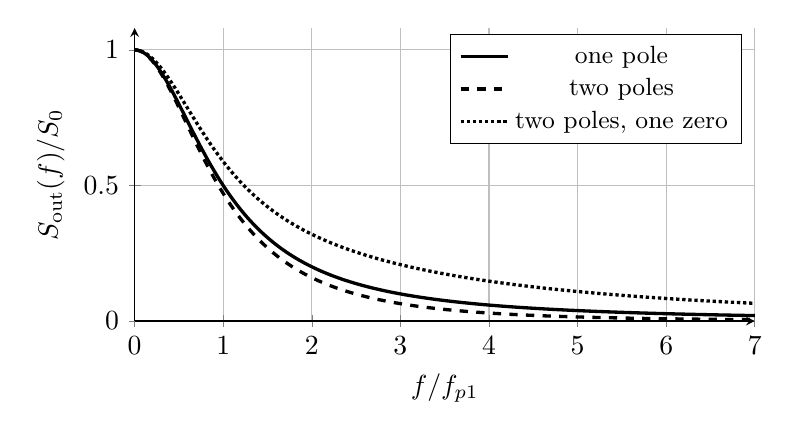
\begin{tikzpicture}
\begin{axis}[width=.78\linewidth,height=5.3cm,axis lines=left,
  xlabel={$f/f_{p1}$},ylabel={$S_{\mathrm{out}}(f)/S_0$},
  xmin=0,xmax=7,ymin=0,ymax=1.08,grid=major,samples=220,
  legend style={at={(.98,.98)},anchor=north east,font=\small}]
  \addplot[black,very thick,domain=0:7] {1/(1+x^2)};
  \addlegendentry{one pole}
  \addplot[black,very thick,dashed,domain=0:7] {1/((1+x^2)*(1+(x/4)^2))};
  \addlegendentry{two poles}
  \addplot[black,very thick,densely dotted,domain=0:7] {(1+(x/2)^2)/((1+x^2)*(1+(x/4)^2))};
  \addlegendentry{two poles, one zero}
\end{axis}\end{tikzpicture}
\caption{Normalized white-noise output spectra for $f_{p2}=4f_{p1}$ and $f_z=2f_{p1}$. A second pole reduces high-frequency area; a zero between the poles increases it.}
\label{fig:multipole}\end{figure}}


\newcommand{\FIRFigure}{%
\begin{figure}[htbp]\centering
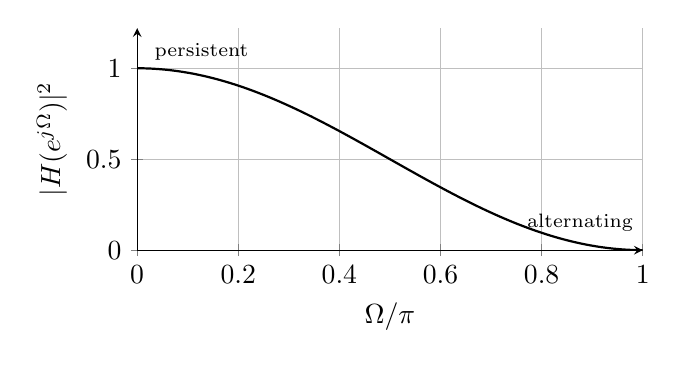
\begin{tikzpicture}
\begin{axis}[width=.66\linewidth,height=4.4cm,xmin=0,xmax=1,ymin=0,ymax=1.22,
 axis lines=left,xlabel={$\Omega/\pi$},ylabel={$|H(e^{j\Omega})|^2$},grid=major]
\addplot[black,thick,domain=0:1,samples=100]{cos(90*x)^2};
\node[font=\scriptsize,anchor=north west] at (axis cs:.015,1.19){persistent};
\node[font=\scriptsize,anchor=south east] at (axis cs:1,.05){alternating};
\end{axis}\end{tikzpicture}
\caption{The two-tap averager has unity gain at DC and a zero at Nyquist. For independent samples, the output variance is half the input variance.}
\end{figure}}

\newcommand{\EnsembleFigure}{%
\begin{figure}[htbp]\centering
\begin{tikzpicture}[x=1cm,y=1cm,>=Latex]
\foreach \y/\lab/\v in {0/s_4/-1,1/s_3/1,2/s_2/-1,3/s_1/1}{
\draw[gray!30] (0,\y)--(8,\y);
\node[left] at (0,\y){$\lab$};
\draw[thick] (.2,{\y+.22*\v})--(7.8,{\y+.22*\v});}
\draw[->,dashed,thick] (3,3.6)--(3,-.6);
\node[below,font=\small] at (3,-.6){ensemble: across outcomes};
\draw[->,thick] (.2,4)--(7.8,4);
\node[above,font=\small] at (4,4){time: along one outcome};
\end{tikzpicture}
\caption{The persistent coin process: every row is a constant $+1$ or $-1$ relative to its own baseline. Averaging many independent records estimates the zero ensemble mean; extending one record leaves its time average unchanged.}
\end{figure}}

\newcommand{\OverlapIntervalsFigure}{%
\begin{figure}[htbp]\centering
\begin{tikzpicture}[x=1cm,y=1cm,>=Latex]
\draw[->](-.5,0)--(8.5,0) node[right]{$u$};
\draw[line width=3pt,black!70] (0,1)--(6,1);
\draw[line width=3pt,black!40] (-1.5,.5)--(4.5,.5);
\draw[<->] (0,-.4)--(4.5,-.4) node[midway,below]{$T-\tau$};
\draw[dashed] (0,-.4)--(0,1.2) (4.5,-.4)--(4.5,1.2);
\node[right,font=\small] at (6.2,1){$u\in I_T$};
\node[right,font=\small] at (4.7,.5){$u+\tau\in I_T$};
\node[below,font=\small] at (2.8,-1){positive shift $0<\tau<T$};
\end{tikzpicture}
\caption{Only the shared interval contains pairs with both $t_2=u$ and $t_1=u+\tau$ inside the recorded window. For a negative shift the same argument gives $T-|\tau|$.}
\end{figure}}


\newcommand{\SpectrumConventionFigure}{%
\begin{figure}[htbp]\centering
\begin{tikzpicture}[x=1cm,y=.95cm]
\begin{scope}
\draw[gray!60](-2.8,0)--(2.8,0) node[right]{$f$};
\fill[black!16](-2.55,0)rectangle(2.55,.35);
\draw[black,thick](-2.55,.35)--(2.55,.35);
\draw[-{Latex[length=2.5mm]},black,very thick](-1.6,0)--(-1.6,1.25);
\draw[-{Latex[length=2.5mm]},black,very thick](1.6,0)--(1.6,1.25);
\draw[-{Latex[length=2.5mm]},black,very thick](0,0)--(0,1.9);
\node[above] at (-1.6,1.35){$A^2/4$};\node[above] at (1.6,1.35){$A^2/4$};
\node[above] at (0,2){$m^2$};
\foreach \x/\lab in {-1.6/-f_0,0/0,1.6/f_0}{\node[below,font=\small]at(\x,-.06){$\lab$};}
\node[font=\small]at(0,-1.05){two-sided floor: $S_W^{(2)}$};
\end{scope}
\begin{scope}[xshift=8cm]
\draw[gray!60](-.6,0)--(3.2,0) node[right]{$f$};
\fill[black!16](0,0)rectangle(2.9,.7);
\draw[black,thick](0,.7)--(2.9,.7);
\draw[-{Latex[length=2.5mm]},black,very thick](0,0)--(0,1.9);
\draw[-{Latex[length=2.5mm]},black,very thick](1.6,0)--(1.6,2.5);
\node[above]at(0,2){$m^2$};\node[above]at(1.6,2.6){$A^2/2$};
\node[below,font=\small]at(0,-.06){$0$};\node[below,font=\small]at(1.6,-.06){$f_0$};
\node[font=\small]at(1.2,-1.05){one-sided floor: $2S_W^{(2)}$};
\end{scope}
\end{tikzpicture}
\caption{Two-sided and one-sided spectra. Shading denotes continuous noise density; arrows denote spectral masses, labeled by their values.}
\label{fig:spectral-masses}\end{figure}}

\newcommand{\RCFigure}{%
\begin{figure}[htbp]\centering
\begin{tikzpicture}[>=Latex]
\draw (0,0)--(5,0); \draw (0,0)--(0,.8);
\draw (0,1.2) circle (.4); \node at (0,1.2){$e_R$};
\draw (0,1.6)--(0,2)--(1.5,2);
\draw[decorate,decoration={zigzag,segment length=4pt,amplitude=1.7pt}](1.5,2)--(2.06,2);
\node[above] at (1.78,2.1){$R$};
\draw (2.06,2)--(5,2);\fill (4,2) circle(1.5pt);
\draw (4,2)--(4,1.18) (3.65,1.18)--(4.35,1.18) (3.65,1.02)--(4.35,1.02) (4,1.02)--(4,0);
\node[right] at (4.4,1.1){$C$}; \node[right] at (5,2){$v_C$};
\end{tikzpicture}
\caption{Resistor noise drives an ideal capacitor through the RC low-pass response.}
\end{figure}}

\newcommand{\NoiseCirclesFigure}{%
\begin{figure}[htbp]\centering
\begin{tikzpicture}[x=3.2cm,y=3.2cm,>=Latex]
\draw[gray!45] (0,0) circle(1);\draw[->,gray!60](-1.1,0)--(1.1,0) node[right,font=\small]{$\operatorname{Re}\Gamma_s$};
\draw[->,gray!60](0,-1.1)--(0,1.1) node[above,font=\small]{$\operatorname{Im}\Gamma_s$};
\foreach \d/\style in {.5/solid,1/dashed,2/densely dotted}{
\pgfmathsetmacro{\Nn}{(pow(10,(2.16+\d)/10)-pow(10,2.16/10))*(1+.36+1.2*cos(83))/(4*.69)}
\pgfmathsetmacro{\cx}{.60*cos(83)/(1+\Nn)}
\pgfmathsetmacro{\cy}{.60*sin(83)/(1+\Nn)}
\pgfmathsetmacro{\rr}{sqrt(\Nn*(1+\Nn-.36))/(1+\Nn)}
\draw[thick,\style] (\cx,\cy) circle(\rr);}
\fill ({.6*cos(83)},{.6*sin(83)}) circle(.018) node[right,font=\small]{$\Gamma_{\mathrm{opt}}$};
\draw[thick] ({.78*cos(108)-.025},{.78*sin(108)-.025})--({.78*cos(108)+.025},{.78*sin(108)+.025});
\draw[thick] ({.78*cos(108)-.025},{.78*sin(108)+.025})--({.78*cos(108)+.025},{.78*sin(108)-.025});
\node[left,font=\small] at ({.78*cos(108)},{.78*sin(108)}){$S_{11}^*$};
\node[font=\small,anchor=west] at (1.3,.7){solid: $NF_{\min}+0.5$ dB};
\node[font=\small,anchor=west] at (1.3,.5){dashed: $NF_{\min}+1$ dB};
\node[font=\small,anchor=west] at (1.3,.3){dotted: $NF_{\min}+2$ dB};
\node[font=\small,anchor=west] at (1.3,-.1){$NF_{\min}=2.16$ dB};
\node[font=\small,anchor=west] at (1.3,-.3){$r_n=0.69$, $Z_0=50\,\Omega$};
\end{tikzpicture}
\caption{Constant noise-figure circles in the reflection-coefficient plane for the illustrative noise parameters. The unit circle bounds passive source impedances. The noise optimum (dot) differs from the unilateral gain optimum (cross).}
\label{fig:noise-circles}\end{figure}}

\newcommand{\CorrelationPairFigure}{%
\begin{figure}[htbp]\centering
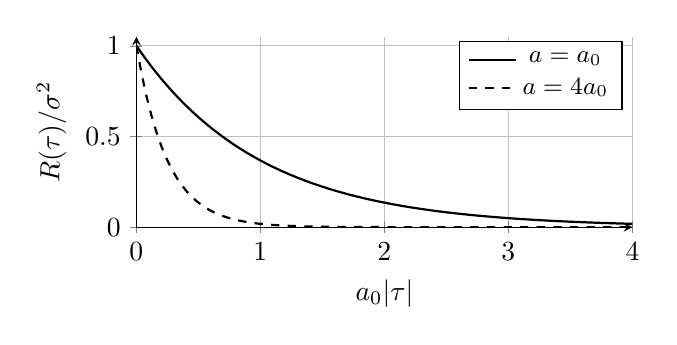
\begin{tikzpicture}
\begin{axis}[width=.65\linewidth,height=4cm,axis lines=left,xlabel={$a_0|\tau|$},ylabel={$R(\tau)/\sigma^2$},xmin=0,xmax=4,ymin=0,ymax=1.05,grid=major,
legend style={font=\small},samples=100]
\addplot[black,thick,domain=0:4]{exp(-x)};\addlegendentry{$a=a_0$}
\addplot[black,thick,dashed,domain=0:4]{exp(-4*x)};\addlegendentry{$a=4a_0$}
\end{axis}\end{tikzpicture}
\caption{The time-domain partner of Figure~\ref{fig:lorentzian}, with $a_0=2\pi f_0$. Shorter correlation time gives a wider PSD while leaving zero-lag variance fixed.}
\end{figure}}


\newcommand{\WKRegionsFigure}{%
\begin{figure}[!ht]\centering
\begin{tikzpicture}[x=2.6cm,y=2.2cm,>=Latex]
\begin{scope}
\fill[black!9](0,0)rectangle(1,1);
\draw[thick](0,0)rectangle(1,1);
\draw[->,gray!70](-.2,0)--(1.35,0)node[right]{$t_2$};
\draw[->,gray!70](0,-.2)--(0,1.35)node[above]{$t_1$};
\draw[dashed](0,0)--(1,1);
\draw[very thick](0,.35)--(.65,1);
\node[font=\small,rotate=40]at(.34,.78){$t_1-t_2=\tau$};
\node[below]at(1,0){$T$};\node[left]at(0,1){$T$};
\node[font=\small]at(.5,-.65){$D:\ 0\leq t_1,t_2\leq T$};
\end{scope}
\draw[->,thick](1.65,.5)--(2.1,.5);
\node[font=\small,align=center]at(1.85,.9){$u=t_2$\\$\tau=t_1-t_2$};
\begin{scope}[xshift=7cm]
\fill[black!9](0,0)--(0,1)--(1,0)--(1,-1)--cycle;
\draw[thick](0,0)--(0,1)--(1,0)--(1,-1)--cycle;
\draw[->,gray!70](-.2,0)--(1.4,0)node[right]{$u$};
\draw[->,gray!70](0,-1.2)--(0,1.35)node[above]{$\tau$};
\draw[very thick](0,.35)--(.65,.35);
\draw[<->] (.02,.55)--(.63,.55)node[midway,above,font=\small]{$T-\tau$};
\node[left]at(0,1){$T$};\node[below right]at(1,0){$T$};
\node[right]at(1,-1){$-T$};
\node[font=\small]at(.5,-1.65){$D':\ 0\leq u\leq T,\ -u\leq\tau\leq T-u$};
\end{scope}
\end{tikzpicture}
\caption{The square of recorded time pairs and its image under the linear change of variables. The bold segment on the left becomes a fixed-$\tau$ horizontal slice on the right. For $\tau>0$ its length is $T-\tau$; for $\tau<0$ it is $T+\tau$.}
\label{fig:wk-regions}\end{figure}}

\newcommand{\InputReferralFigure}{%
\begin{figure}[htbp]\centering
\begin{tikzpicture}[>=Latex]
\node[draw,minimum width=3.2cm,minimum height=1.2cm,align=center](net)at(5,0){linear network\\signal transfer $H_s(f)$};
\draw[->](0,0)--(net.west)node[midway,above]{$u_s$};
\draw[->](net.east)--(10,0)node[midway,above]{$y_s+y_n$};
\node[font=\small,align=center]at(1.5,-1){input reference:\\voltage $v_s$ or current $i_s$};
\node[font=\small,align=center]at(8.7,-1){output PSD $S_{y_n}$\\same measured output};
\node[font=\small,align=center]at(5,-2.1){$S_{u,\mathrm{eq}}=S_{y_n}/|H_s|^2$\\$H_s=y_s/v_s$ for voltage; $H_s=y_s/i_s$ for current};
\end{tikzpicture}
\caption{Input-referred noise reproduces the output PSD through the specified voltage or current signal transfer.}
\label{fig:input-referral}\end{figure}}

\newcommand{\TwoPortFigure}{%
\begin{figure}[!ht]\centering
\begin{tikzpicture}[x=.9cm,y=.9cm,>=Latex]
\draw[dashed,gray!75,rounded corners=2pt](-1.1,-.4)rectangle(5.9,3.25);
\node[font=\small,above]at(2.4,3.3){input network};
\draw (0,0)--(6.3,0);\draw (0,0)--(0,.8);
\draw (0,1.15)circle(.35);\node[left]at(-.45,1.15){$v_s$};
\node[font=\scriptsize]at(0,1.3){$+$};\node[font=\scriptsize]at(0,1){$-$};
\draw (0,1.5)--(0,2.2)--(1.2,2.2);
\draw (1.2,2)rectangle(2.1,2.4);\node[above]at(1.65,2.45){$Z_s$};
\draw (2.1,2.2)--(2.75,2.2);
\draw (3.1,2.2)circle(.35);\node[above]at(3.1,2.65){$e_n$};
\node[font=\scriptsize]at(2.92,2.2){$-$};\node[font=\scriptsize]at(3.28,2.2){$+$};
\draw (3.45,2.2)--(6.3,2.2);
\draw (4.7,0)--(4.7,.8);\draw (4.7,1.15)circle(.35);
\draw[->](4.7,.93)--(4.7,1.37);\draw (4.7,1.5)--(4.7,2.2);
\node[right]at(5.15,1.15){$i_n$};
\fill(4.7,2.2)circle(1.5pt);\fill(4.7,0)circle(1.5pt);
\draw[dashed,<->](3.4,2.7)to[bend left=22](4.7,1.7);
\node[font=\small,above]at(4.8,2.75){$S_{ie}$};
\draw (6.3,-.3)rectangle(8.8,2.5);
\node[align=center]at(7.55,1.1){noiseless\\two-port};
\draw (8.8,2.2)--(10.2,2.2)--(10.2,1.6);
\draw (10,.7)rectangle(10.4,1.6);\draw (10.2,.7)--(10.2,0)--(8.8,0);
\node[right]at(10.5,1.15){$Z_L$};\node[above]at(9.5,2.3){$v_o$};

\end{tikzpicture}
\caption{Equivalent input voltage and current noise; the dashed network is converted to Norton form below.}
\label{fig:two-port}\end{figure}}

\newcommand{\NortonNoiseFigure}{%
\begin{figure}[!ht]\centering
\begin{tikzpicture}[x=.8cm,y=.85cm,>=Latex]
\draw[dashed,gray!75,rounded corners=2pt](-1.35,-.4)rectangle(6.8,3.05);
\node[font=\small,above]at(2.9,3.1){Norton equivalent};
\draw (0,0)--(8,0);\draw (0,2.5)--(8,2.5);
\foreach \x/\lab in {0/i_s,4/i_a}{
\draw (\x,0)--(\x,.9);\draw (\x,1.3)circle(.4);\draw[->](\x,1.05)--(\x,1.55);\draw (\x,1.7)--(\x,2.5);
}\node[left]at(-.45,1.3){$i_s$};\node[right]at(4.45,1.3){$i_a$};
\draw (2,0)--(2,.8);\draw (1.8,.8)rectangle(2.2,1.7);\draw (2,1.7)--(2,2.5);
\node[below]at(2,.65){$Y_s$};
\draw (8,-.3)rectangle(11,2.8);\node[align=center]at(9.5,1.25){noiseless\\two-port};
\draw[->](11,2.5)--(12.3,2.5)node[right]{$y_o$};\draw (11,0)--(12.3,0);
\node[font=\small,align=center]at(5.5,-1.05){$i_a=i_n+Y_se_n$\\source: $S_{i_s}=4kT_0G_s$};
\end{tikzpicture}
\caption{Input Norton equivalent: source noise $i_s$ and added noise $i_a$ drive the same node.}
\label{fig:norton-noise}\end{figure}}

\newcommand{\ProjectionFigure}{%
\begin{figure}[htbp]\centering
\begin{tikzpicture}[>=Latex]
\node[draw,minimum width=2.1cm,minimum height=1.05cm,align=center](yc)at(3,1){$Y_c(f)$\\\small scale and phase};
\node[draw,circle,minimum size=.65cm,inner sep=0pt](add)at(6.5,1){$+$};
\draw[->](0,1)--(yc.west)node[midway,above]{$e_n$};
\draw[->](yc.east)--(add.west)node[midway,above]{$Y_ce_n$};
\node[font=\small,align=center]at(5.1,1.9){correlated\\current};
\draw[->](6.5,-1)--(add.south)node[midway,right]{$i_u$};
\node[font=\small,align=center]at(4.6,-.65){uncorrelated\\remainder};
\draw[->](add.east)--(9.5,1)node[midway,above]{$i_n$};
\node[font=\small]at(5,-1.5){$S_i=|Y_c|^2S_e+S_u$,\qquad $S_{i_ue}=0$};
\end{tikzpicture}
\caption{The current noise is a voltage-correlated component plus an uncorrelated remainder.}
\label{fig:projection}\end{figure}}

\newcommand{\AdmittanceCancellationFigure}{%
\begin{figure}[htbp]\centering
\begin{tikzpicture}[x=2.5cm,y=1.5cm,>=Latex]
\draw[->,gray!70](-.4,0)--(2,0)node[right]{$G$ (mS)};
\draw[->,gray!70](0,-1.5)--(0,1.6)node[above]{$B$ (mS)};
\draw[->,thick](0,0)--(0,1)node[left]{$Y_c=j1$};
\draw[->,thick](0,0)--(1,-1)node[below right]{$Y_s=1-j1$};
\draw[->,very thick](0,0)--(1,0)node[midway,above]{$Y_s+Y_c=1$};
\draw[->,dashed](1,-1)--(1,0)node[midway,right,font=\small]{$+Y_c$};
\node[below left,font=\small]at(0,0){$0$};
\end{tikzpicture}
\caption{Source susceptance cancels the imaginary part of $Y_s+Y_c$ in the numerical example.}
\label{fig:admittance-cancellation}\end{figure}}

\newcommand{\FriisFigure}{%
\begin{figure}[htbp]\centering
\begin{tikzpicture}[>=Latex]
\foreach \x/\j in {2.5/1,6/2,9.5/3}{
\node[draw,minimum width=1.8cm,minimum height=1.1cm,align=center](g\j)at(\x,0){stage $\j$\\$G_{T,\j}$, $F_\j$};
\draw[->](\x,-1.8)--(\x,-.6);
\node[font=\small,align=center]at(\x,-2.25){added at input\\$A_\j=(F_\j-1)kT_0B$};}
\draw[->](0,0)--(g1.west);\node[font=\small]at(.45,.75){$N_s=kT_0B$};
\draw[->](g1.east)--(g2.west);\draw[->](g2.east)--(g3.west);
\draw[->](g3.east)--(12,0)node[right]{$N_o$};
\node[font=\small]at(6,-3.1){input referral: $A_1$,\quad $A_2/G_{T,1}$,\quad $A_3/(G_{T,1}G_{T,2})$};
\end{tikzpicture}
\caption{Matched cascade with independent stage-added noise. Each $A_j$ is referred to its own stage input, before the gain.}
\label{fig:friis}\end{figure}}

\newcommand{\PhaseNoiseFigure}{%
\begin{figure}[htbp]\centering
\begin{tikzpicture}[x=1cm,y=1cm,>=Latex]
\begin{scope}
\fill[black!12] (0,0) -- plot[domain=0:3.8,samples=80] (\x,{1.8/(1+\x*\x)}) -- (3.8,0) -- cycle;
\draw[gray!60](0,0)--(4.2,0)node[right]{$f$};
\draw[gray!60](0,0)--(0,2.2)node[above]{$S_\phi^{(1)}$};
\draw[thick,domain=0:3.8,samples=80]plot(\x,{1.8/(1+\x*\x)});
\node[font=\small]at(2,-.5){phase spectrum: positive offsets};
\end{scope}
\draw[->,thick](4.9,1)--(5.6,1)node[midway,above,font=\small]{$/2$};
\begin{scope}[xshift=9cm]
\fill[black!12] (-2.3,0) -- plot[domain=-2.3:2.3,samples=100] (\x,{.9/(1+\x*\x)}) -- (2.3,0) -- cycle;
\draw[gray!60](-2.5,0)--(2.5,0)node[right]{$f-f_c$};
\draw[thick,domain=-2.3:2.3,samples=100]plot(\x,{.9/(1+\x*\x)});
\draw[-{Latex[length=2.5mm]},very thick](0,0)--(0,2.2);
\node[above,font=\small]at(0,2.3){carrier mass $1$};
\node[font=\small]at(0,-.5){each RF sideband: $\mathcal L=S_\phi^{(1)}/2$};
\end{scope}
\end{tikzpicture}
\caption{Small phase fluctuations produce two RF noise sidebands. The right plot shows one-sided RF noise normalized to carrier power, with frequency measured relative to the positive carrier.}
\label{fig:phase-noise}\end{figure}}

\newcommand{\MeanErrorRegionsFigure}{%
\begin{figure}[htbp]\centering
\begin{tikzpicture}[scale=.85,font=\small]
\begin{scope}
\fill[black!9] (0,0)--(4,0)--(4,4)--cycle;
\draw[black!45] (0,0) rectangle (4,4);
\draw[thick] (0,0)--(4,4);
\draw[-{Latex}] (0,0)--(4.5,0) node[right] {$t$};
\draw[-{Latex}] (0,0)--(0,4.5) node[above] {$u$};
\node[below] at (4,0) {$T$};\node[left] at (0,4) {$T$};
\node at (2.9,1.1) {$u\leq t$};\node at (1.1,2.9) {$t\leq u$};
\node[below] at (2,-.65) {Original square: equal halves};
\end{scope}
\draw[-{Latex},thick] (4.8,2)--(6.1,2) node[midway,above] {$\tau=t-u$};
\begin{scope}[xshift=7cm]
\fill[black!9] (0,0)--(4,0)--(4,4)--cycle;
\draw[thick] (0,0)--(4,0)--(4,4)--cycle;
\draw[-{Latex}] (0,0)--(4.5,0) node[right] {$t$};
\draw[-{Latex}] (0,0)--(0,4.5) node[above] {$\tau$};
\draw[very thick] (1.5,1.5)--(4,1.5);
\node[below] at (2.75,1.5) {$T-\tau$};
\node[left] at (0,1.5) {$\tau$};\node[below] at (4,0) {$T$};
\node[below] at (2,-.65) {Transformed triangle: $\tau\leq t\leq T$};
\end{scope}
\end{tikzpicture}
\caption{Even covariance gives equal contributions from the two halves of the original square. Transforming the lower half to $(t,\tau)$ gives a triangle. At fixed lag $\tau$, the horizontal interval has length $T-\tau$.}
\label{fig:mean-regions}\end{figure}}

\newcommand{\CorrelationAveragingFigure}{%
\begin{figure}[htbp]\centering
\begin{tikzpicture}
\begin{axis}[width=.47\linewidth,height=4cm,xmin=0,xmax=12,ymin=-3.5,ymax=3.5,
title={Short correlation: $\tau_c=0.4t_0$},title style={font=\small},
xlabel={$t/t_0$},ylabel={$X(t)/\sigma$},tick label style={font=\scriptsize},label style={font=\small}]
\addplot[black,thin] table[x=t,y=fast]{figures/correlation_averaging_data.dat};
\addplot[black!45,dashed,domain=0:12]{0};
\end{axis}
\begin{scope}[xshift=7.9cm]
\begin{axis}[width=.47\linewidth,height=4cm,xmin=0,xmax=12,ymin=-3.5,ymax=3.5,
title={Long correlation: $\tau_c=4t_0$},title style={font=\small},
xlabel={$t/t_0$},tick label style={font=\scriptsize},label style={font=\small}]
\addplot[black,thin] table[x=t,y=slow]{figures/correlation_averaging_data.dat};
\addplot[black!45,dashed,domain=0:12]{0};
\end{axis}\end{scope}
\begin{scope}[yshift=-4.7cm]
\begin{axis}[width=.47\linewidth,height=4.2cm,xmin=0,xmax=12,ymin=0,ymax=1.1,
title={Model autocovariance},title style={font=\small},xlabel={$\tau/t_0$},
ylabel={$C_X(\tau)/\sigma^2$},tick label style={font=\scriptsize},label style={font=\small},
legend style={font=\scriptsize,at={(.5,-.53)},anchor=north,legend columns=3,draw=none,fill=none}]
\addplot[black,thick,domain=0:12,samples=120]{exp(-x/.4)};\addlegendentry{Short}
\addplot[black,thick,dashed,domain=0:12,samples=120]{exp(-x/4)};\addlegendentry{Long}
\addplot[black,densely dotted,thick,domain=0:12]{1};\addlegendentry{Persistent}
\end{axis}\end{scope}
\begin{scope}[xshift=7.9cm,yshift=-4.7cm]
\begin{axis}[width=.47\linewidth,height=4.2cm,xmin=0,xmax=12,ymin=0,ymax=1.1,
title={Mean-estimation error},title style={font=\small},xlabel={$T/t_0$},
ylabel={$\operatorname{MSE}(T)/\sigma^2$},tick label style={font=\scriptsize},label style={font=\small}]
\addplot[black,thick,domain=.005:12,samples=150]{2*.4/x*(1-.4/x*(1-exp(-x/.4)))};
\addplot[black,thick,dashed,domain=.005:12,samples=150]{2*4/x*(1-4/x*(1-exp(-x/4)))};
\addplot[black,densely dotted,thick,domain=0:12]{1};
\end{axis}\end{scope}
\end{tikzpicture}
\caption{Stationary Gaussian records with equal variance and different correlation times. The lower panels compare their model covariances and exact mean-estimation MSEs with those of a persistent random offset. Time is normalized by $t_0$.}
\label{fig:correlation-averaging}\end{figure}}

\newcommand{\PeriodogramScatterFigure}{%
\begin{figure}[!htbp]\centering
\begin{tikzpicture}
\begin{axis}[width=.88\linewidth,height=3.0cm,xmin=0,xmax=.125,ymin=0,ymax=10,
title={One record: $N=256$},title style={font=\small},
ylabel={$I/S_0$},xticklabels=\empty,tick label style={font=\scriptsize},label style={font=\small}]
\addplot[black,thin] table[x=f,y=psd]{figures/periodogram_short.dat};
\addplot[black!55,dashed,domain=0:.125]{1};
\end{axis}
\begin{scope}[yshift=-3.25cm]
\begin{axis}[width=.88\linewidth,height=3.0cm,xmin=0,xmax=.125,ymin=0,ymax=10,
title={One record: $N=4096$},title style={font=\small},
ylabel={$I/S_0$},xticklabels=\empty,tick label style={font=\scriptsize},label style={font=\small}]
\addplot[black,thin] table[x=f,y=psd]{figures/periodogram_long.dat};
\addplot[black!55,dashed,domain=0:.125]{1};
\end{axis}\end{scope}
\begin{scope}[yshift=-6.5cm]
\begin{axis}[width=.88\linewidth,height=3.0cm,xmin=0,xmax=.125,ymin=0,ymax=10,
title={Average of 32 independent records: $N=4096$ each},title style={font=\small},
xlabel={$f\Delta t$},ylabel={$I/S_0$},xtick={0,.025,.05,.075,.1,.125},xticklabels={0,0.025,0.05,0.075,0.10,0.125},scaled x ticks=false,tick label style={font=\scriptsize},label style={font=\small}]
\addplot[black,thin] table[x=f,y=psd]{figures/periodogram_averaged.dat};
\addplot[black!55,dashed,domain=0:.125]{1};
\end{axis}\end{scope}
\end{tikzpicture}
\caption{FFT periodograms of independent, unit-variance Gaussian samples on common axes. The dashed line is the true normalized PSD. A longer record narrows bin spacing; averaging 32 independent records reduces scatter. The flat source spectrum has no window bias at these FFT bins.}
\label{fig:periodogram-scatter}\end{figure}}

\newcommand{\MixerImageNoiseFigure}{%
\begin{figure}[!htbp]\centering
\begin{tikzpicture}[x=.88cm,y=.85cm,>=Latex,font=\small]
  \node[anchor=west,font=\bfseries\small] at (0,4.8) {RF input};
  \draw[->,gray] (0,3.25)--(12.4,3.25) node[right] {$f_{\mathrm{RF}}$};
  \fill[black!12] (2.15,3.25) rectangle (3.45,3.95);
  \draw[dashed,thick] (2.15,3.25)--(2.15,3.95)--(3.45,3.95)--(3.45,3.25);
  \fill[black!12] (8.55,3.25) rectangle (9.85,3.95);
  \draw[thick] (8.55,3.25)--(8.55,3.95)--(9.85,3.95)--(9.85,3.25);
  \draw[->,very thick] (9.2,3.25)--(9.2,4.65);
  \node[above] at (2.8,4.05) {image noise};
  \node[above] at (9.2,4.65) {desired signal};
  \node[anchor=west,font=\footnotesize] at (9.95,3.65) {noise};
  \draw[densely dotted] (6,3.05)--(6,4.35);
  \node[below] at (6,3.2) {$f_{\mathrm{LO}}$};
  \node[below] at (2.8,3.2) {$f_{\mathrm{LO}}-f_{\mathrm{IF}}$};
  \node[below] at (9.2,3.2) {$f_{\mathrm{LO}}+f_{\mathrm{IF}}$};
  \draw[->,thick,dashed] (2.8,2.65) to[out=-75,in=145] (5.6,1.05);
  \draw[->,thick] (9.2,2.65) to[out=-105,in=35] (6.4,1.05);
  \node[fill=white,inner sep=2pt] at (6,2.1) {$f_{\mathrm{IF}}=|f_{\mathrm{RF}}-f_{\mathrm{LO}}|$};
  \node[anchor=west,font=\bfseries\small] at (0,.75) {IF output};
  \draw[->,gray] (2,-.3)--(11.8,-.3) node[right] {$f$};
  \fill[black!12] (5.35,-.3) rectangle (6.65,.2);
  \fill[black!28] (5.35,.2) rectangle (6.65,.7);
  \draw[thick] (5.35,-.3) rectangle (6.65,.7);
  \draw[dashed] (5.35,.2)--(6.65,.2);
  \draw[->,very thick] (6,-.3)--(6,1.35);
  \node[below] at (6,-.35) {$f_{\mathrm{IF}}$};
  \node[anchor=west,font=\footnotesize] at (7,.55) {image noise: $G_c kT_0B$};
  \node[anchor=west,font=\footnotesize] at (7,-.05) {desired-band noise: $G_c kT_0B$};
  \node[anchor=east,font=\footnotesize] at (5.05,1.1) {signal: $G_cP_s$};
  \node[anchor=west] at (0,-1.25) {Equal conversion gains: total IF noise $=2G_ckT_0B$.};
\end{tikzpicture}
\caption{Noise from the desired and image bands adds at IF; shading shows the two contributions.}
\label{fig:mixer-image-noise}
\end{figure}}

\newcommand{\CorrelationSpectrumFigure}{%
\begin{figure}[htbp]\centering
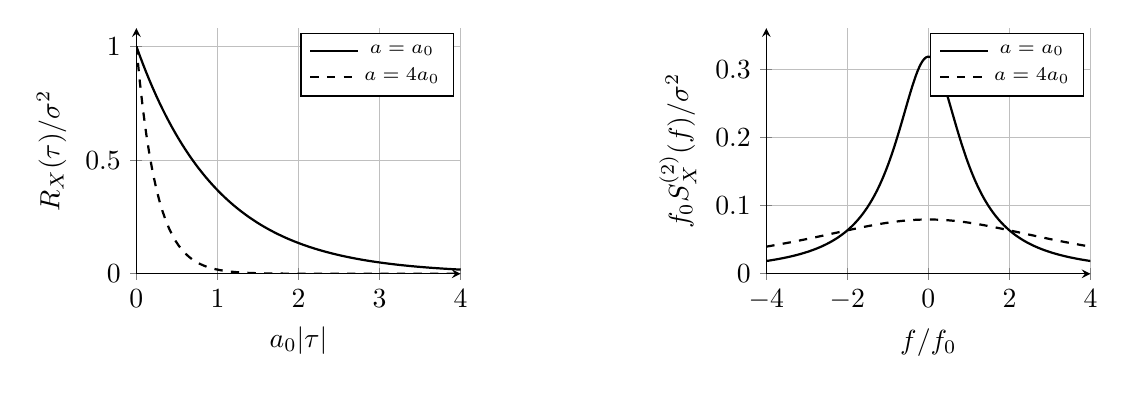
\begin{tikzpicture}
\begin{axis}[width=.47\linewidth,height=4.7cm,axis lines=left,
xlabel={$a_0|\tau|$},ylabel={$R_X(\tau)/\sigma^2$},
xmin=0,xmax=4,ymin=0,ymax=1.08,grid=major,
legend style={font=\scriptsize,at={(.98,.98)},anchor=north east},samples=100]
\addplot[black,thick,domain=0:4]{exp(-x)};\addlegendentry{$a=a_0$}
\addplot[black,thick,dashed,domain=0:4]{exp(-4*x)};\addlegendentry{$a=4a_0$}
\end{axis}
\begin{scope}[xshift=8.0cm]
\begin{axis}[width=.47\linewidth,height=4.7cm,axis lines=left,
xlabel={$f/f_0$},ylabel={$f_0S_X^{(2)}(f)/\sigma^2$},
xmin=-4,xmax=4,ymin=0,ymax=.36,grid=major,samples=200,
legend style={font=\scriptsize,at={(.98,.98)},anchor=north east}]
\addplot[black,thick,domain=-4:4]{1/(pi*(1+x^2))};\addlegendentry{$a=a_0$}
\addplot[black,thick,dashed,domain=-4:4]{4/(pi*(16+x^2))};\addlegendentry{$a=4a_0$}
\end{axis}\end{scope}
\end{tikzpicture}
\caption{Correlation and its Lorentzian spectrum, with $a_0=2\pi f_0$. Faster decorrelation broadens the spectrum while preserving the variance.}
\label{fig:lorentzian}\end{figure}}
